% These packages are optional, depending whether you want the features they provide.
% See the LaTeX Companion or other references for full information.
% !TEX TS-program = pdflatex
% !TEX encoding = UTF-8 Unicode

% This is a simple template for a LaTeX document using the "article" class.
% See "book", "report", "letter" for other types of document.

\documentclass[12pt]{article} % use larger type; default would be 10pt
\usepackage[T2A]{fontenc}
\usepackage[utf8]{inputenc} % set input encoding (not needed with XeLaTeX)
\usepackage[russian]{babel}
%%% Examples of Article customizations
% These packages are optional, depending whether you want the features they provide.
% See the LaTeX Companion or other references for full information.

%%% PAGE DIMENSIONS
\usepackage{geometry}

\usepackage{fancyhdr} 
\geometry{a4paper} % or letterpaper (US) or a5paper or....
% \geometry{margin=2in} % for example, change the margins to 2 inches all round
% \geometry{landscape} % set up the page for landscape
%   read geometry.pdf for detailed page layout information
\usepackage{sectsty}
\usepackage{graphicx} % support the \includegraphics command and options
\usepackage{mathtext}
\usepackage{amsmath}
\usepackage{amsfonts}
\usepackage{mathtools}

\newcommand\myeq{\stackrel{\rm Def}{=}}
% \usepackage[indentfill]{indentskip} % Activate to begin indentagraphs with an empty line rather than an indent
\usepackage{biblatex}
\usepackage{hyperref}
\hypersetup{
  colorlinks=true,
  linkcolor=blue,
  urlcolor=green
}
%%% END Article customizations

%%% The "real" document content comes below...
\usepackage{setspace}

\usepackage{listings}
\lstset{
	breaklines=true,
	tabsize=2,
}
%%% ToC (table of contents) APPEARANCE
\usepackage[nottoc,notlof,notlot]{tocbibind} % Put the bibliography in the ToC
\usepackage[titles,subfigure]{tocloft} % Alter the style of the Table of Contents

%\date{} % Activate to display a given date or no date (if empty),
         % otherwise the current date is printed 
\usepackage{physics}
\usepackage{float}
\begin{titlepage}
	\begin{center}
	\large{МИНОБРНАУКИ РОССИИ}\\
	\footnotesize{ФЕДЕРАЛЬНОЕ ГОСУДАРСТВЕННОЕ БЮДЖЕТНОE ОБРАЗОВАТЕЛЬНОЕ УЧРЕЖДЕНИЕ}\\ 
	\footnotesize{ВЫСШЕГО ПРОФЕССИОНАЛЬНОГО ОБРАЗОВАНИЯ}\\
	\small{\textbf{«САНКТ-ПЕТЕРБУРГСКИЙ ГОСУДАРСТВЕННЫЙ ПОЛИТЕХНИЧЕСКИЙ УНИВЕРСИТЕТ ПЕТРА ВЕЛИКОГО»}}\\
	\hfill \break
	\normalsize{Институт компьютерных наук и технологий}\\
	\hfill \break
	\normalsize{Высшая школа искусственного интеллекта}\\
	\hfill\break
	\begin{center}
		\normalsize{Дисциплина: \\ТЕОРИЯ ГРАФИИ}
	\end{center}
	\hfill \break
	\hfill \break
	\large{ОТЧЕТ}\\
	\large{Лабораторная работа №0:}\\
	\large{«КОДИРОВАНИЕ»}\\
	\hfill \break
	\hfill \break
	\hfill \break
	\hfill \break
	\hfill \break
	\hfill \break
\end{center}	

\normalsize{ 
	\begin{tabular}{ccc}
		Обучающийся &  гр. 3530201/10001 & Нгуен Куок Дат \\\\
		Руководитель & \hrulefill 				& Востров Алексей Владимирович\\\\
	\end{tabular}
}\\
\hfill \break
\hfill \break
\hfill \break
\hfill \break
\begin{center} Санкт-Петербург 2022 
\end{center}
\end{titlepage}
\usepackage{indentfirst}
\begin{document}
\begin{center}
\input{titlepage}
\end{center}
\doublespacing
\tableofcontents
\newpage
\section*{Введение}
\addcontentsline{toc}{section}{Введение}
	В данной работе необходимо реализовать шифратор и дешифратор для данных алгoритм: Фано и RLE, применяющиеся на текстовый файл 10000 символов. Программно кодировать и декодировать алгоритимами Фано, RLE и также применять двухстепенчатое кодирование; одновременно необходимо определить цену кодирования и коэффициент сжатия. 
\newpage
\section{Матиматическое описание}
\subsection{Кодирование}
\subsubsection{Алфавитное кодирование}
Алфавитное (или побуквенное) кодирование задается схемой (или таблицей кодов) $\sigma$ 
\[ \sigma \,\myeq\, \langle a_1 \rightarrow \beta_1, \dots a_n \rightarrow \beta_n \rangle, \quad a_i \in A, \beta_i \in B^*,\] где$\beta_i $ - кодовое слово. 

Алфавитное кодирование пригодно для любого множества сообщений \textit{S}:
\[ F: A^* \rightarrow B^*,\quad\quad\quad a_{i_1} \dots a_{i_k} = \alpha \in A*, \quad\quad\quad F(\alpha) =\beta_{i_1}\dots\beta_{i_k}\] 
\subsubsection{Разделимые и префиксные схемы}
Схема $\sigma$ называется \textit{разделимой}, если
\[ \beta_{i_1}\dots\beta_{i_k} = \beta_{j_1}\dots\beta_{j_l} \implies k= l \& \forall t\in 1..k (i_t = j_t)\]
то есть любое слово, составленное из элементарных кодов, единственным образом разлагается на элементарные коды. Алфавитное кодирование с разделимой схемой допускает декодирование.

Схема $\sigma$ называется префиксной, если элементарный код одной буквы не является префиксом элементарного кода другой буквы: 
\[ \neg \exist \beta_i , \beta_j \in V, \beta \in B^* (i\neq j \quad\&\quad \beta_i = \beta_j\beta)\]
Префиксная схема является разделимой, поэтому допускает декодирование. 

\subsubsection{Цена кодирования}
Заданы алфавит $А = \{a_1,...,a_n \}$ и вероятности появления букв в сообщении $P = \langle p_i,\dots ,p_n\rangle$ ($p_i$ — вероятность появления буквы $a_i$). Не ограничивая общности, можно считать, что $ p_1 + \dots + p_n = 1$ и $p_1 \geq \dots \geq p_n > 0$.

Для каждой разделимой схемы $\sigma = \langle a_i \rightarrow \beta_i \rangle ^n _{i=1}$ алфавитного кодирования математическое ожидание коэффицеинта увеличения длины сообщения при кодировании $\sigma$ называется  средней \textit{ценой кодирования $\sigma$} при распределении вероятностей $P$:
\[ l_\sigma (P) \,\,\myeq\,\, \sum^n_{i=1}{p_i \lvert \beta_i\rvert}\]

\newpage
\subsection{Алгоритм Фано}
Рекурсивный алгоритм Фано строит разделимую префиксную схему алфавитного кодирования, близкого к оптимальному.\\ 
\textbf{Ввод: } частото-убывающий алфавит, начало, конец, кодовая схема\\
\textbf{Вывод: } кодовая схема (словарь)
\begin{figure}[H]
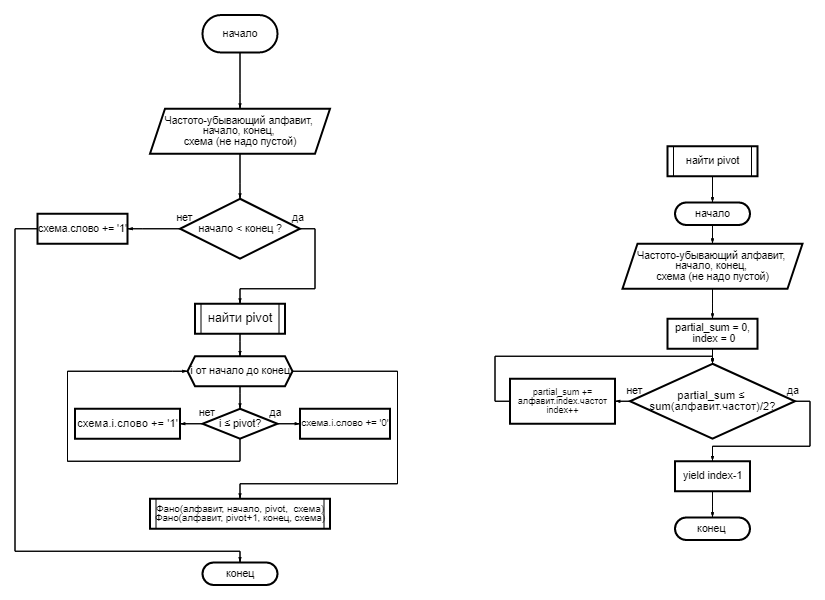
\includegraphics[scale =0.5]{fano.png}
\caption{Блок-схема алгоритма Фано}
\end{figure}
\newpage
\subsection{Алгоритм RLE}
Алгоритм RLE \textit{run-length encoding} - заменяет строку одинаковых символов строкой, содержащей сам повторяющийся символ и количество его повторов.

В этой программe, чтобы избежать использования слишком большого объема данных, если серия имеет больше 255 символов (тогда надо по крайней мере 2 char сохранящие кратность), она будет <<выделена>>. \\
\textbf{Ввод: } частото-убывающий алфавит, начало, конец, кодовая схема\\
\textbf{Вывод: } кодовая схема (словарь)\\
\begin{figure}[H]
\centering 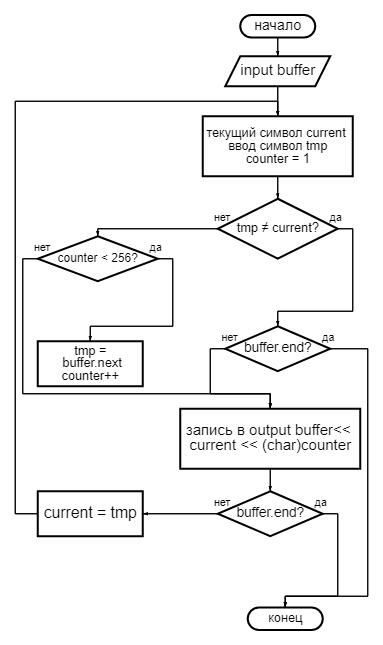
\includegraphics[scale =0.75]{rle.png}
\caption{Блок-схема алгоритма RLE}
\end{figure}
\newpage
\section{Реализация}
\subsection{Текстовый генератор}
Используя генератор для случаных чисел (\textit{rand()}), выберяют характер по индексу из данной списки.  \\

\noindent \textbf{Вход: } Объём файл (10000 характеров), списка символов\\
\textbf{Выход: }  Текстовый файл \\

\subsection{Битовая упаковка}
Один главный процедур это битовая упаковка. Поскольку система не позволяет нам напрямую работать с битами, закодированные данные нужно <<упаковуют>> в строке, чтобы сжать более эффективно. 

При отображении с байтов на битов, данные могут быть не кратен байтам, поэтому в конце шифорванной строки нужны несколько <<заполненных>> битов (padding bit). Одновременно, другая проблема возникает: нулевый характер в конце строки будет пропущен, которое приводит к потере данных. Чтобы решить эту задачу, добавляют один байт в концу, которому назначен количество заполненных битов. 

Так как упаковка (и распаковка) работают с битами, файл должно быть открыт в \textit{binary mode}, чтобы избегать то, что данные меняются. \\
\textbf{Вход: }Последовательность шифруемых символов S, словарь D. \\
\textbf{Выход: } Строка упаковки. 
 \begin{figure}[H]
\centering 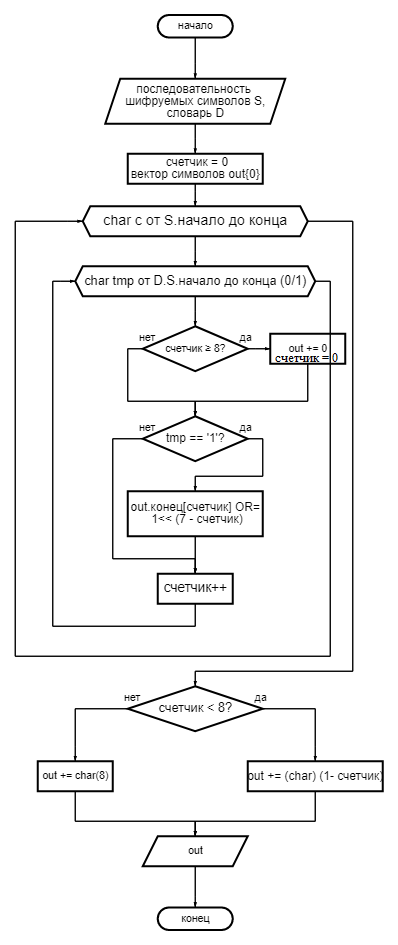
\includegraphics[scale =0.75]{pack.png}
\caption{Блок-схема битовой упаковки}
\end{figure}
\newpage
\subsection{Дешифрование}
\subsubsection{Для RLE}
Для RLE-шифрованных данных не нужен словарь, только читать символы и переписывать данные.\\ 
\textbf{Вход: }Последовательность шифрованных символов S\\
\textbf{Выход: }Строка перивичных данных \\
 \begin{figure}[H]
\centering 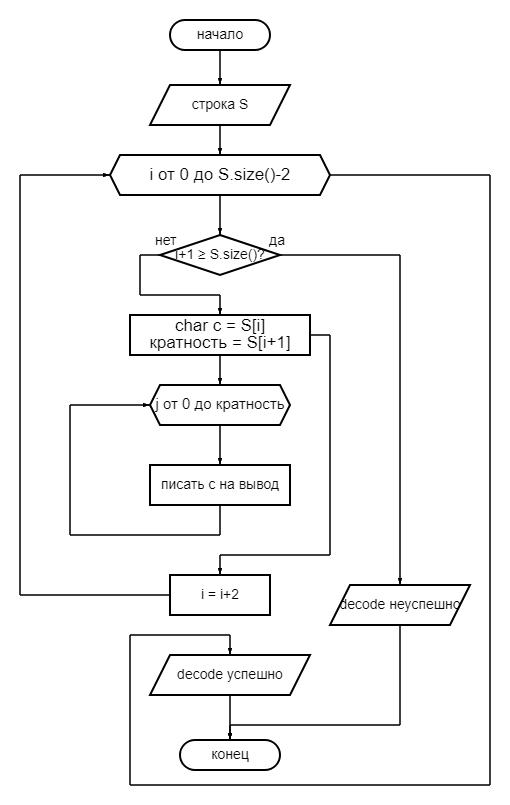
\includegraphics[scale =0.4]{decoderle.png}
\caption{Блок-схема дешифрования для RLE}
\end{figure}
\subsubsection{Для Фано}
Для Фано-шифорванных данных нужны внешний словарь и процедура <<распаковки>>. \\
\textbf{Вход: }Последовательность шифрованных символов S, словарь D\\
\textbf{Выход: } Строка перивичных данных \\
 \begin{figure}[H]
\centering 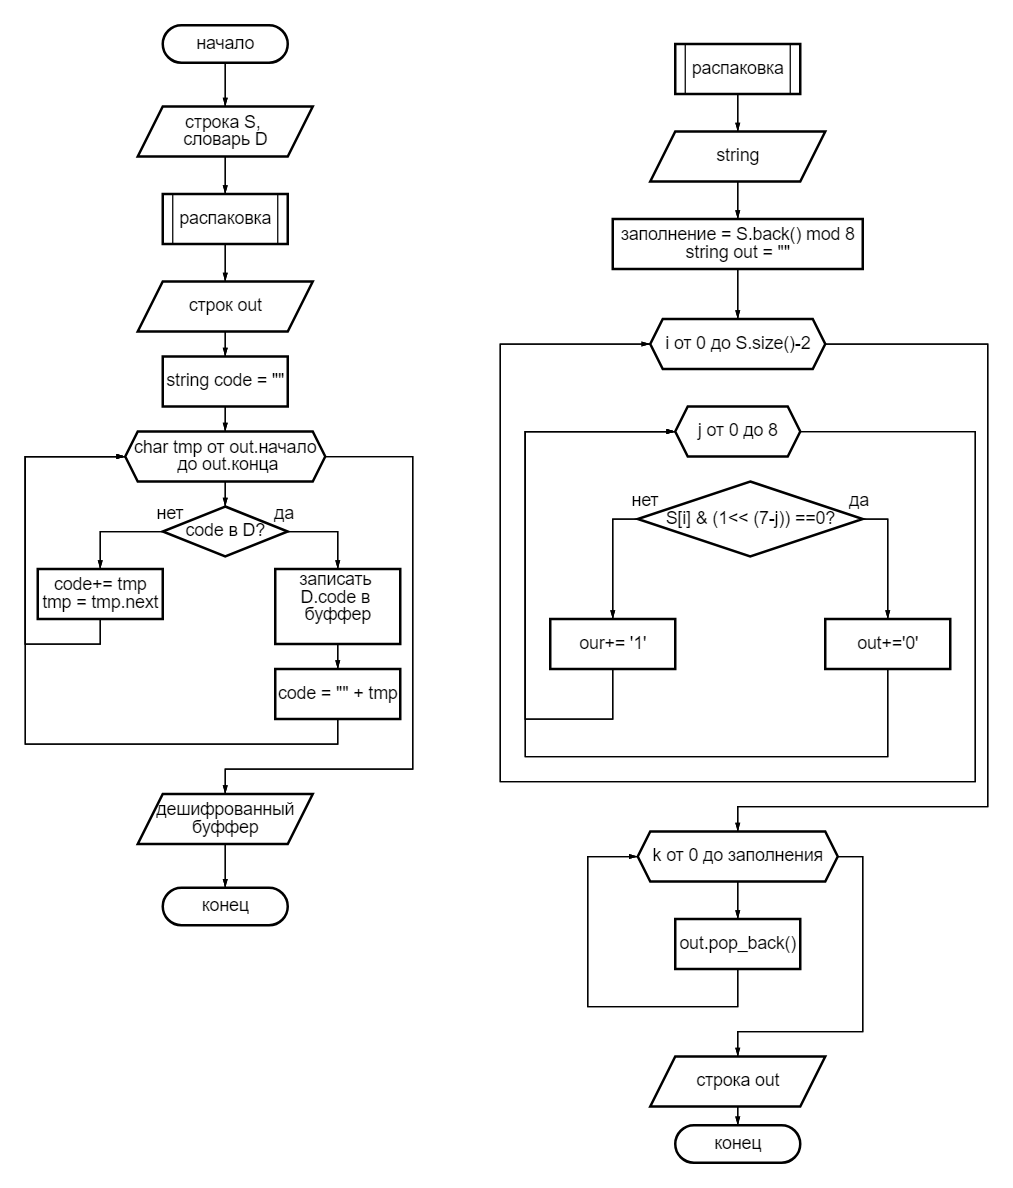
\includegraphics[scale =0.33]{decodefano.png}
\caption{Блок-схема дешифрования для Фано}
\end{figure}
\subsection{Проверка дешифрованных данных}
Данные проверят по символам,  внутри функции сравнение 2 строки. Если они равны, то дешифрованние нормально работает. \\
\textbf{Вход: }2 строки\\
\textbf{Выход: } 0 если равны, другие если не равны \\

\subsection{Вычисление коэффициента сжатия}
\[\text{ коэффициент сжатия} = \frac{\text{Объём исходных данных}}{\text{Объём шифрованных данных}}\]
\textbf{Вход: }2 строки \\
\textbf{Выход: }Вывод коэффициент сжатия на экран \\

\newpage
\section{Результат работы}
 \begin{figure}[H]
\centering
\begin{subfigure}
\centering
 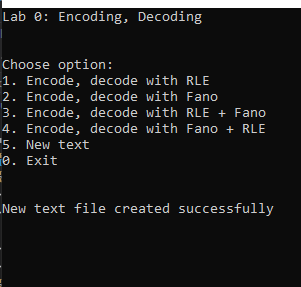
\includegraphics[scale = 0.8]{textcreated.png}
\end{subfigure}
\hfill
\begin{subfigure}
\centering 
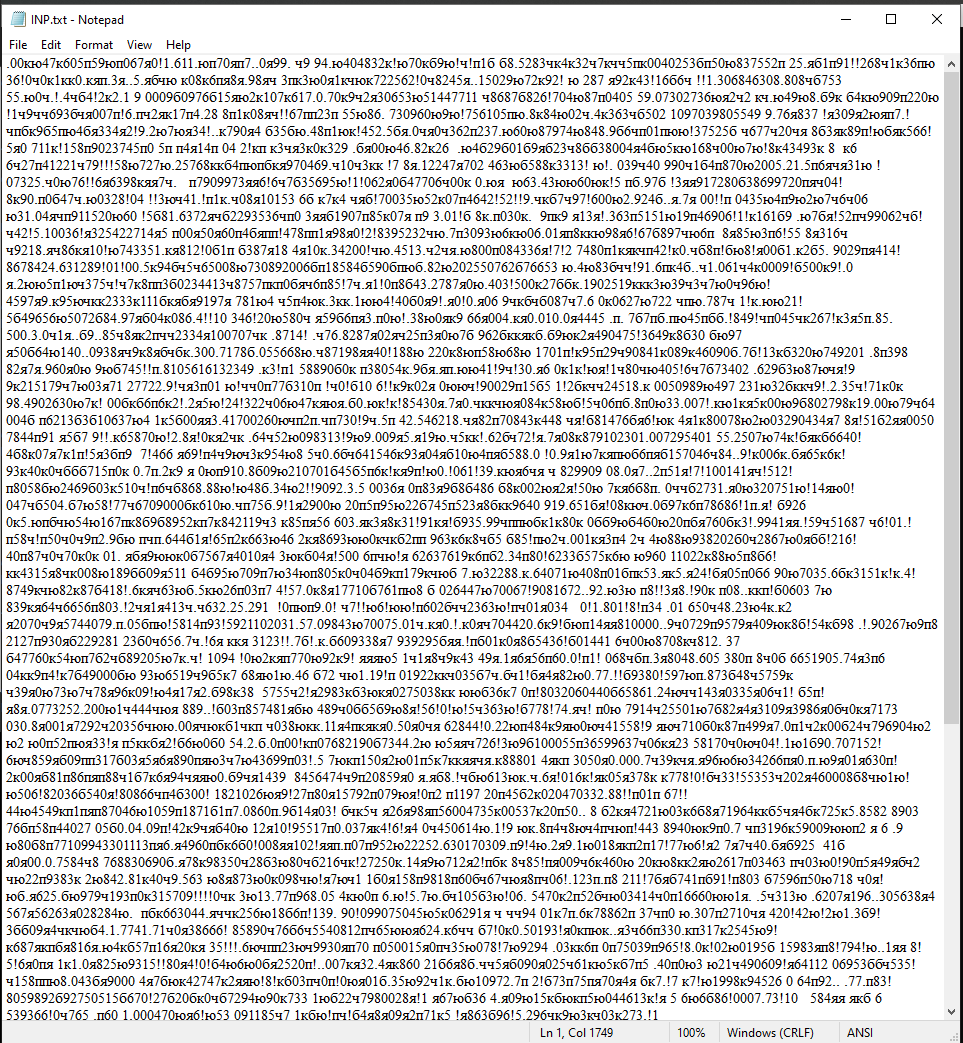
\includegraphics[scale = 0.3]{inp.png}
\end{subfigure}
\caption{Новый текст файл созданый} \label{text}
\end{figure}
В р \ref{text}, новый текст \textbf{INP.txt} с 10000 символов создан. 

 \begin{figure}[H]
\centering
\begin{subfigure}
\centering
 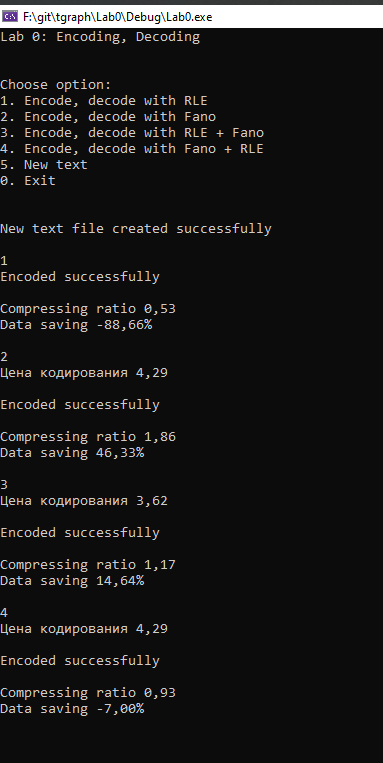
\includegraphics[scale = 0.5]{coded.png}
\end{subfigure}
\hfill
\begin{subfigure}
\centering 
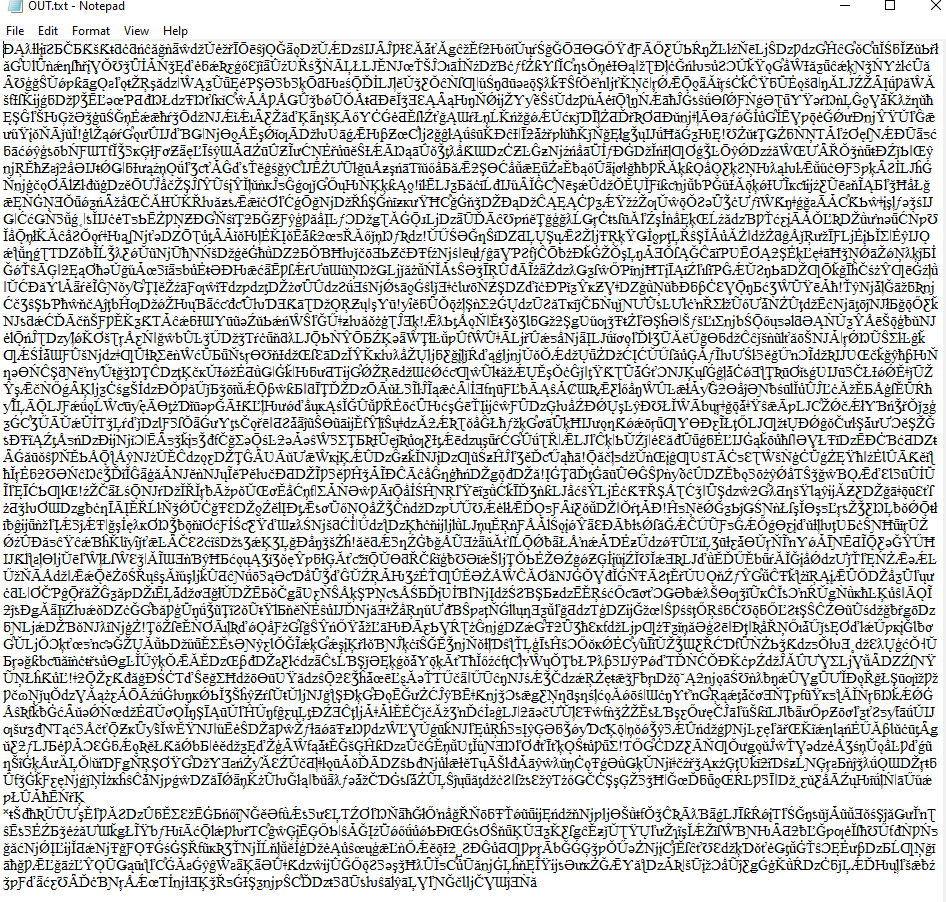
\includegraphics[scale = 0.3]{out.png}
\end{subfigure}
\caption{Шифрование} \label{code}
\end{figure}
В рисунке \ref{code}, характеры в \textbf{INP.txt} шифруются и записываются в \textbf{OUT.txt}. Цену кодирования и коэффициенты сжатия вычислены. 

Видимо, что RLE-шифорвание увеличивает объём файла. Однако, Фано-шифрование сжает файл на ~50\%. 

Сравнивая двухстепенчатые RLE-Фано и Фано-RLE шифрования, можем заключить, что с данной файлом, RLE-Фано шифрование более эффективно.

\begin{figure}[H]
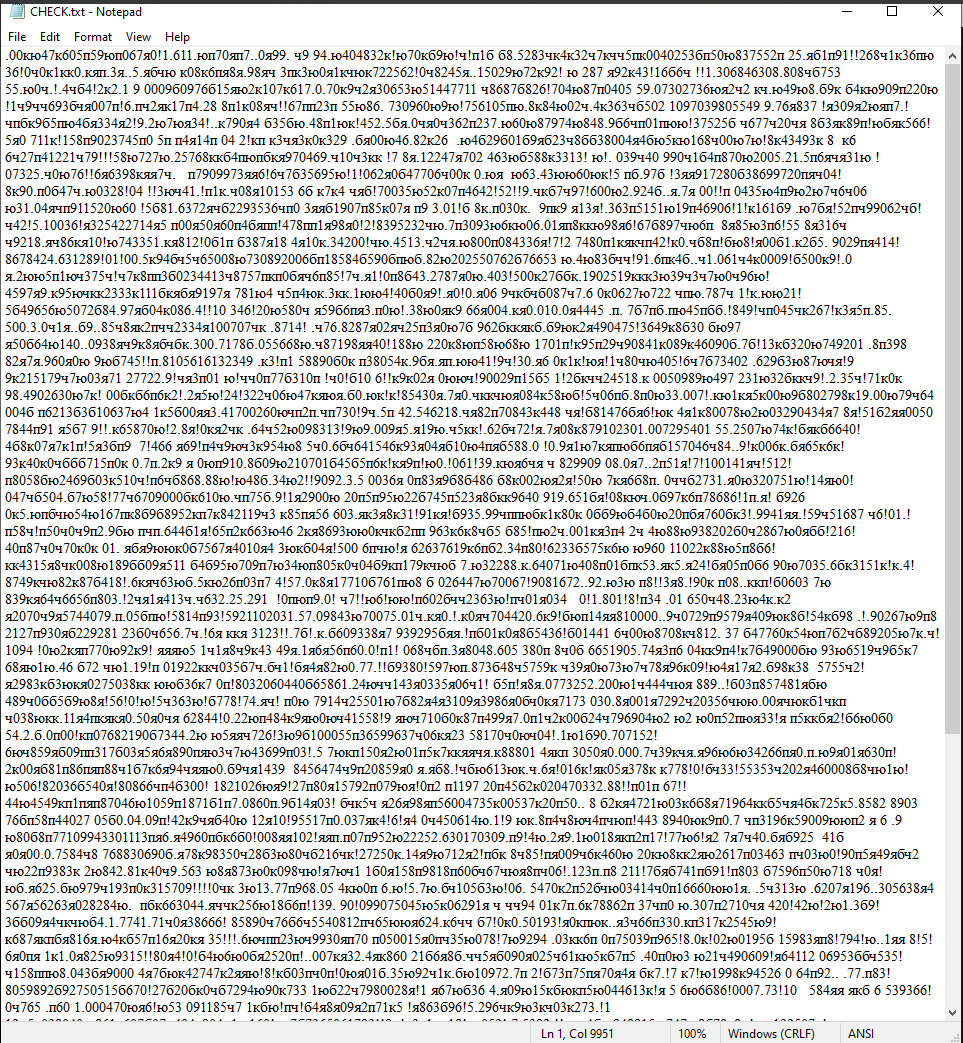
\includegraphics[scale = 0.5]{check.png}
\caption{Дешифрование} \label{decode}
\end{figure}
В рисунке \ref{decode}, дешифруемые данные записываются в \textbf{check.txt}


\newpage
	\section*{Заключение}
		\addcontentsline{toc}{section}{Заключение}
	 В данной работы успешно написана программа, реализующая шифратор и дешифратор с алгоритмами Фано, RLE и соответственными двухстепечатыми. Шифрование и дешифрование произошлы, цена кодирования и коэффициенты сжатия определены. Видимо, что Фано-шифрование самое эффективное, и двухстепенчатое RLE-Фано шифрование более эффективно, чем Фано-RLE шифрование. 
	
	 Преимущества программы заключаются в том, что реализация в общем виде, для любой списки символов. С идеями о битовой 	упаковке и распаковке могут создать функцию в отдельную библиотеку для других целей. 
	
	 Недостаток программы заключается в том, что исходный код не оптимизирован, особенно с алгоритмом RLE: шифрованные данные больше исходных. Процедуры упаковки и распаковки написаны внутри функции шифрования, значит им надо переписывать, иначе не могут повторно использовать. 
	
	 Данная лабораторная работа была реализована на языке C++ в среде программирования Visual Studio 2019.
\newpage
\begin{thebibliography}{3}
\bibitem{Novikov}
Ф.А. Новиков «Дискретная математика для программистов: Учебник для вузов». 3-е издание.- СПБ.: Питер, 2009. -384 с.: ил. - (Серия <<Учебник для вузов>>)

День обращения: 10.02.2023

\bibitem{Lectures}
 Конспект лекций Вострова А.В по дискретной математике.

День обращения: 10.02.2023

\bibitem{RLE} 
Алгоритм RLE
\url{https://en.wikipedia.org/wiki/Run-length_encoding}

День обращения: 10.02.2023
\end{thebibliography}

\end{document}